\documentclass{article}

% Language setting
% Replace `english' with e.g. `spanish' to change the document language
\usepackage[portuguese]{babel}

% Set page size and margins
% Replace `letterpaper' with`a4paper' for UK/EU standard size
\usepackage[letterpaper,top=2cm,bottom=2cm,left=3cm,right=3cm,marginparwidth=1.75cm]{geometry}

% Useful packages
\usepackage{amsmath}
\usepackage{graphicx}
\usepackage[colorlinks=true, allcolors=blue]{hyperref}
\usepackage{subfig}
\usepackage{verbatim}

\title{MEI - Milestone 1\\Exploratory Data Analysis and Linear Regression}
\author{Gonçalo São Marcos 2018284198\\
        José Esperança 2018278596}

\begin{document}

\begin{titlepage}
   \begin{center}
       \vspace*{1cm}
    
        
    {\huge \textbf{\textit{MEI - Milestone 1\\Exploratory Data Analysis and Linear Regression}}}
       
        \vspace{0.7cm}

        Professor Luís Filipe dos Santos Coelho Paquete\\Metodologias Experimentais em Informática - MEI 2021/2022
            
        \vspace{0.7cm}
        \textbf{Gonçalo São Marcos, 2018284198\\
                José Esperança, 2018278596\\}

        \vspace{0.4cm}
        Contactos: \\
        \href{mailto:gmarcos.dei.uc.pt}{gmarcos@student.dei.uc.pt}\\
        \href{mailto:esperanca.dei.uc.pt}{esperanca@student.dei.uc.pt}
        
        \vspace{4.6cm}
        
\includegraphics[width=0.3\textwidth]{dei.png}
        \vfill
        Mestrado em Engenharia Informática\\
       Departamento de Engenharia Informática\\
       Universidade de Coimbra\\
       Portugal\\
       09 de novembro de 2021
            
   \end{center}
\end{titlepage}


\pagebreak

\section{Introdução}
\paragraph{}
No âmbito da unidade curricular de Metodologias Experimentais em Informática, foi-nos proposto desenhar uma experiência com o intuito de avaliar o desempenho de um programa que gere o escalonamento de exames no Departamento de Engenharia Informática.
O objetivo principal é a exploração do método experimental apresentado, seguindo os passos sugeridos, testando, observando e realizando uma análise dos resultados, de forma a retirarmos conclusões sobre este programa. O programa em causa é-nos fornecido pelo docente em duas versões que resolvem o mesmo problema, apresentando implementações diferentes, acompanhadas por um gerador de dados de entrada que permite obter os dados simulados necessários para correr os programas. Deste modo, o nosso objetivo para esta primeira meta passa por desenhar as experiências, testar os dois programas, observar os dados obtidos e, como mencionado anteriormente, tirar conclusões fundamentadas pelo processo experimental que nos ajudem nas próximas metas deste trabalho prático. O \textit{Problem Statement} também nos é descrito em detalhe no enunciado do trabalho prático pelo que, inicialmente, este foi analisado com cuidado, de modo a entender melhor o problema em causa e, consequentemente, conseguirmos gerar hipóteses coerentes acerca do comportamento do programa.\par
Tratando-se da primeira meta do trabalho prático, apenas nos é pedido que realizemos uma análise exploratória aos resultados obtidos e que sejam realizadas algumas regressões lineares que achemos relevantes para que, nas próximas etapas, avancemos com a definição de hipóteses e os seus respetivos testes.\par
O presente documento deverá descrever o nosso processo de desenho da experiência com detalhe suficiente para permitir a reprodução do mesmo, como solicitado no enunciado.



\section{Identificação das variáveis}
\paragraph{}
Analisado o \textit{Problem Statement}, focamos a nossa atenção nos dois programas fornecidos, no seu código, no gerador de dados de entrada e nas variáveis que estes programas necessitam para executar, de forma a identificarmos no nosso problema as variáveis que nos irão ser úteis no desenvolvimento desta experiência.
Começando pelo programa que gera os dados de entrada (\textit{gen.py}), este recebe como variáveis de entrada o \textbf{número de exames}, a \textbf{probabilidade (p) de cada par de exames ter um estudante em comum}, uma \textbf{semente aletória} e o \textbf{nome do ficheiro} onde os dados gerados serão guardados e que será o ficheiro de input dos programas.\par
Ambos os programas (\textit{code1.c} e \textit{code2.c}) necessitam dos mesmos argumentos para serem executados: uma \textbf{semente aleatória}, o \textbf{tempo máximo de execução} do programa (após o qual o programa interrompe a execução e devolve um valor de erro) e o \textbf{nome do ficheiro de dados de entrada} que foi previamente gerado.\par
A partir do \textit{Problem Statement}, verificamos que a variável que queremos medir e avaliar é o \textbf{tempo de execução do programa}, ou seja, o tempo que o programa demora a encontrar, ou não, uma solução para determinados dados de entrada. Isto é verdade pois este tempo para a obtenção de uma solução é um aspeto importante para potenciais clientes destes programas e, por isso mesmo, considerámos esta variável como sendo a nossa única \textbf{variável dependente}. Os fatores que alteram o tempo de execução do programa, ou seja, que influenciam a variável dependente, serão as nossas \textbf{variáveis independentes}. Identificámos o \textbf{número de exames} e a \textbf{probabilidade (p) de cada par de exames ter um estudante em comum} como sendo as nossas \textbf{variáveis independentes} pelo facto de serem estes argumentos do gerador de dados de entrada que alteram o tempo que os programas demoram a encontrar, ou não, uma solução.\par

Sumarizando, temos:
\begin{description}
   \item[Variável dependente] Tempo de execução do programa.
   \item[Variáveis Independentes] Número de exames; Probabilidade (p) de cada par de exames ter um estudante em comum
\end{description}

\section{Fase Experimental e de Observação}
\paragraph{}
Identificadas as variáveis relevantes no contexto do nosso problema, passamos agora à fase mais prática da nossa experiência. De seguida serão abordadas as experiências em si e toda a preparação necessária para a realização das mesmas, tal como os resultados que fomos observando ao longo dos diversos testes.

\subsection{Configuração das Experiências}
\paragraph{}
De modo a avaliar a influência das variáveis independentes no tempo de execução dos programas optámos por uma abordagem iterativa onde, em cada iteração, é gerado um novo ficheiro de dados de entrada (\textit{data.in}, recorrendo ao \textit{gen.py}) e ambos os programas (\textit{code1.c} e \textit{code2.c}) são executados sequencialmente, sendo que o \textit{output} é guardado num ficheiro de texto para posterior análise no programa R. Em cada iteração é alterado o valor da variável independente em análise para mais tarde conseguirmos analisar, com recurso a gráficos, a dependência que queremos estudar. É importante referir que cada iteração é executada \textit{N} vezes, dependendo do grau de precisão que pretendemos obter numa determinada experiência. Isto é feito com o objetivo de reduzir potenciais variações no tempo de execução influenciados por eventuais fatores externos como o escalonamento do processo no CPU, programas a correr em simultâneo, semente aleatória, etc. As sementes aleatórias também foram sempre renovadas antes de cada iteração através de um número aleatório gerado pela \textit{GNU Bash}. \par
Todos os testes foram realizados numa máquina com as seguintes características:
\begin{table}[!htbp]
\begin{center} 
\begin{tabular}{ | c | c | } 
  \hline
  CPU & Intel(R) Core(TM) i7-9750H CPU @ 2.60GHz \\ 
  \hline
  GPU & NVIDIA GeForce RTX 2060 \\
  \hline
  RAM & 16,0 GB @ 2667MHz \\
  \hline
  SSD & WD SDAPMUW-512G 512GB PC SN520 \\
  \hline
  OS & Windows 11 Home 21H2 22000.282 a correr WSL2 Ubuntu 20.04.3 LTS\\
  \hline
  GCC & Versão 9.3.0\\
  \hline
  Python & Versão 3.8.10\\
  \hline
  R & Versão 4.1.1\\
  \hline
  RStudio & Versão 1.4.1717\\
  \hline
  GNU Bash & Versão 5.0.17(1)-release\\
  \hline
\end{tabular}
\caption{Hardware e software utilizado}
\end{center}
\end{table}
\subsection{Ferramentas e processos utilizados para a realização das experiências}
\paragraph{}
Decidimos recorrer à \textit{GNU Bash} do Ubuntu visto que, para realizar cada iteração da experiência, tinhamos apenas que executar os três programas \textit{gen.py}, \textit{code1.c} e \textit{code2.c} e guardar os resultados dos últimos dois. Isto é possível, sem exigir grande complexidade de programação, através de um script (\textit{script.sh}) que, recorrendo a ciclos \textit{for}, itera por um determinado vetor de valores para cada uma das variáveis e chama cada programa com esses valores. No fim de cada execução, os \textit{outputs} de cada programa, juntamente com os parâmetros utilizados, são escritos para um ficheiro de texto para armazenamento.

Após o desenho geral do \textit{script}, é possível alterar as suas variáveis de forma a fazer experiências. Por exemplo, podemos fixar o valor do Número de Exames a 20 e percorrer valores de 1\% a 100\% para a Probabilidade (p), testando cada iteração \textit{N} vezes. No final teremos, para cada valor de probabilidade, \textit{N} testes com o valor do tempo de execução do programa. A partir daqui podemos calcular gráficos, médias, desvios padrões, regressões lineares, etc. de forma a analisar os resultados obtidos.

\subsection{Realização das experiências}
\paragraph{}
Inicialmente começámos por, manualmente, fazer alguns testes com valores de Número de Exames e Probabilidade (p) que achávamos relevantes de modo a vermos com que valores os programas se tornavam demasiado lentos para serem executados numa experiência iterativa. Chegámos à conclusão que o Número de Exames poderia tomar valores na casa das dezenas (até 70/80 por exemplo) caso a Probabilidade (p) fosse relativamente baixa (menor que 30\%) sem que o programa se tornasse muito lento. Também observámos o contrário, caso o Número de Exames tomasse um valor mais reduzido, conseguiamos testar, em tempo útil, valores de Probabilidade (p) muito mais elevados. Caso ambas as variáveis tomassem valores muito elevados, os programas demoravam demasiado tempo a encontrar a solução pelo que esse cenário não seria viável para a realização de testes iterativos. Também chegámos a um consenso de que iriamos definir o \textbf{tempo máximo de execução} dos programas em 120 segundos de forma a podermos realizar centenas/milhares de iterações sem que esgotassemos o tempo antes da entrega do trabalho prático. Importante frisar que este valor do tempo máximo pode não representar outliers mas sim uma instância do programa que simplesmente não conseguiu obter a solução em tempo útil pelo que estes valores serão incluídos nos gráficos. Iremos voltar a tocar neste ponto dos valores do tempo máximo nos resultados obtidos no \textbf{Ponto 4}.\par
Com as descobertas acima descritas, passámos à realização de testes automatizados, começando por realizar uma experiência onde o valor para a Probabilidade (p) se encontrava fixa a 20\% e o Número de Exames variava entre 2 e 60, de 2 em 2, sendo que cada iteração era realizada 40 vezes pelas razões mencionadas no ponto \textbf{3.1}. O resultado deste teste pode ser observado na \textbf{Figura 2} apenas como exemplo da representação gráfica do \textit{output} de uma experiência - neste caso um \textit{Scatter Plot} do Tempo de Execução em função do Número de Exames.

\begin{figure} [!htbp]
    \centering
    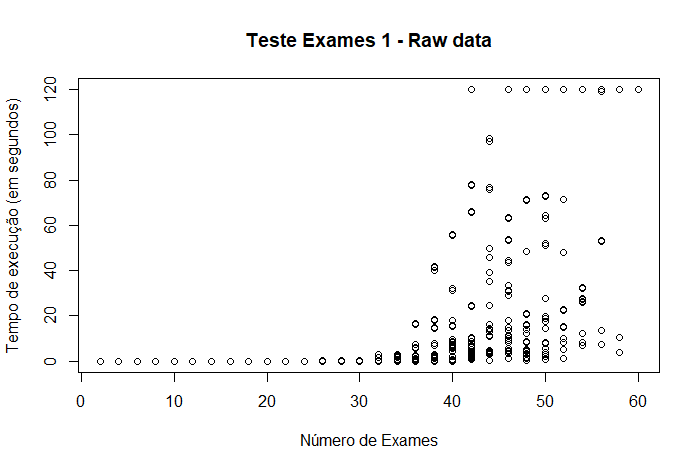
\includegraphics[width=0.7\textwidth]{testeExames_raw.png}
    \caption{Exemplo de resultados de uma experiência}
    \label{fig:testeExames_raw}
\end{figure}

Na \textbf{Tabela 2} podem ser observadas todas as experiências que foram realizadas e como foram sendo alteradas as variáveis de modo a gerar novos resultados. De notar que cada combinação foi testada tanto no programa \textit{code1.c} como no \textit{code2.c}.\par
\begin{description}
   \item[Nota:] Na \textbf{Tabela 2} é usada uma notação de intervalos de iteração [a:b:c] onde \textbf{\textit{a}} representa o início do intervalo, \textbf{\textit{c}} representa o fim do intervalo e \textbf{\textit{b}} o valor do incremento a cada iteração (e.g. [0:2:10] representa o vetor de valores [0,2,4,6,8,10]). A tabela também contém uma coluna \textbf{Id} de forma a mais facilmente podermos fazer referência a cada experiência de forma inequívoca ao longo deste relatório.
\end{description}

\begin{table}[h]
\centering
\begin{tabular}{| c | c | c | c |}\hline

\textbf{Id} & \textbf{Número de Exames} & \textbf{Probabilidade (p) (em \%)} &  \textbf{Número de Repetições} \\ \hline                              

1 & [2:2:60] & 20 & 40\\ \hline

2 & 20 & [2:2:96] & 40\\ \hline

3 & [35:1:60] & 20 & 60\\ \hline

4 & 20 & [65:1:95] & 40\\ \hline

5 & [10:2:60] & [2, 5, 10, 25, 50] & 20\\ \hline

6 & [10:1:40] & [1:1:16] & 20\\ \hline

\end{tabular}
\caption{Experiências realizadas}
\end{table}

\section{Análise dos resultados obtidos}
\paragraph{}
Os testes apresentados na \textbf{Tabela 2} foram sendo feitos sequencialmente, pela ordem apresentada, ou seja, a decisão da realização de uma experiência pode ter sido influênciada pela realização de uma experiência anterior. Este é o caso para as experiências 1 e 3 dado que nesta última o objetivo era obter maior resolução nos resultados obtidos para o intervalo de 35 a 60 exames.\par

Começando pela experiência 1, cujo \textit{output} do \textit{code1.c} pode ser visualizado na \textbf{Figura 2}, podemos observar que, para um valor baixo de probabilidade (20\%), o tempo de execução do programa é quase instantâneo até aos 30 exames. A partir desse ponto é possível ver um grande crescimento no resultado para cada valor de Número de Exames testado o que indica que existe uma tendência para o aumento do tempo de execução.\par

É possível observar que a partir dos 42 exames começam a existir valores do tempo de execução iguais a 120 segundos o que significa que o tempo limite da experiência foi atingido e, portanto, o programa terminou e devolveu um valor de erro, não tendo encontrado a solução dentro do tempo estipulado. Estes casos em que o valor limite para o tempo de execução é alcançado consideramos como um resultado válido (i.e. não se trata necessáriamente de um outlier) pois os dados de entrada para o programa podem realmente não ter uma solução e, tanto o gerador como o programa em si, dependem de sementes aleatórias que podem causar estes resultados onde parece que o programa, por mais tempo que passe, não encontra a solução.\par

Apesar de um \textit{Scatter Plot} ser uma boa ferramenta de visualização dos resultados no seu estado mais puro, não nos transmite muita informação concreta sobre o comportamento do programa pelo que optámos por calcular a média do tempo de execução para cada valor de Número de Exames testado e visualizar esse gráfico. Como se pode observar no gráfico \textbf{(a)} da \textbf{Figura 2}, o uso do valor médio dos resultados para cada valor de Número de Exames permite visualizar muito melhor o crescimento do tempo de execução em função do aumento da variável independente. No entanto, como se verificou na observação dos dados antes de efetuar a média, existe uma grande dispersão dos valores obtidos para cada valor da variável independente, o que sugere que o desvio padrão destes resultados também vá crescendo à medida que o Número de Exames cresce. Esse comportamento pode ser observado no gráfico \textbf{(b)} da \textbf{Figura 2}. Este aumento na variância pode ter que haver com o facto de existir uma componente aleatória nos programas o que por vezes pode levar a resultados muito mais velozes e, noutras vezes, a resultados muito piores que o valor médio. Não observámos nenhuma ligação direta que confirmasse esta teoria mas achamos ser uma ideia que vale a pena investigar em trabalho futuro.\par
De notar que o valor do desvio padrão no gráfico \textbf{(b)} da \textbf{Figura 2} de 0 segundos para o último valor da variável independente deve-se ao facto de, para o valor de 60 exames, todos os resultados terem atingido o limite máximo de tempo (120 segundos) portanto, não existiu qualquer variação entre os valores obtidos.

\begin{figure} [!htbp]
    \centering
    \subfloat[\centering Evolução do tempo de execução]{{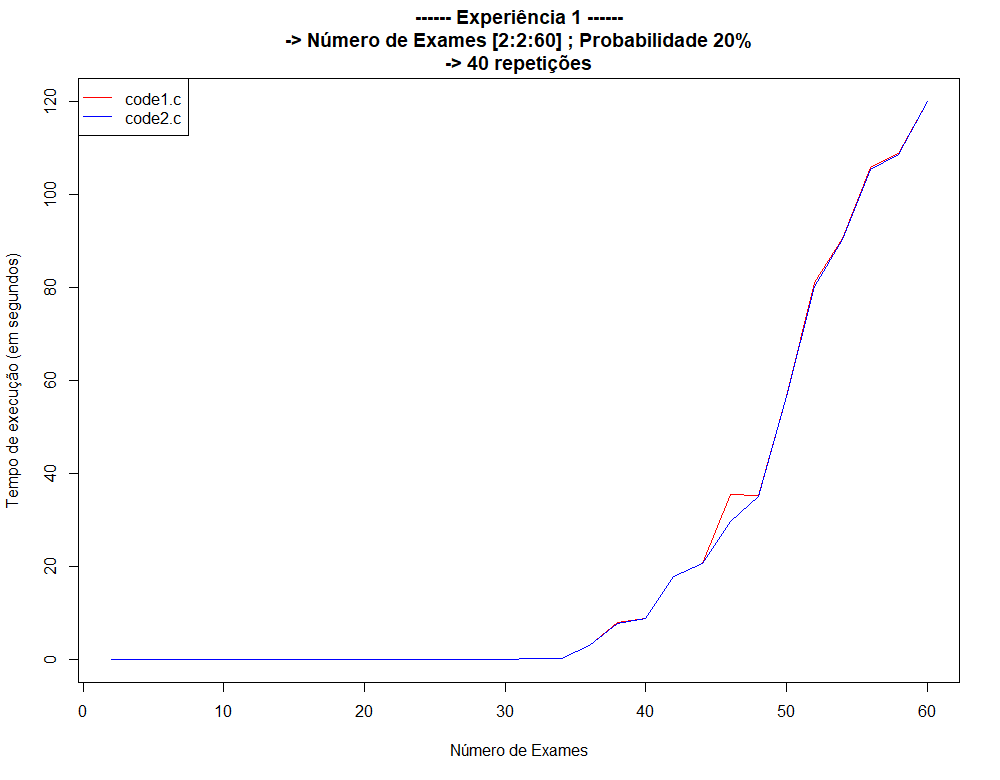
\includegraphics[width=7.3cm]{1_media.png} }}%
    \qquad
    \subfloat[\centering Evolução do desvio padrão]{{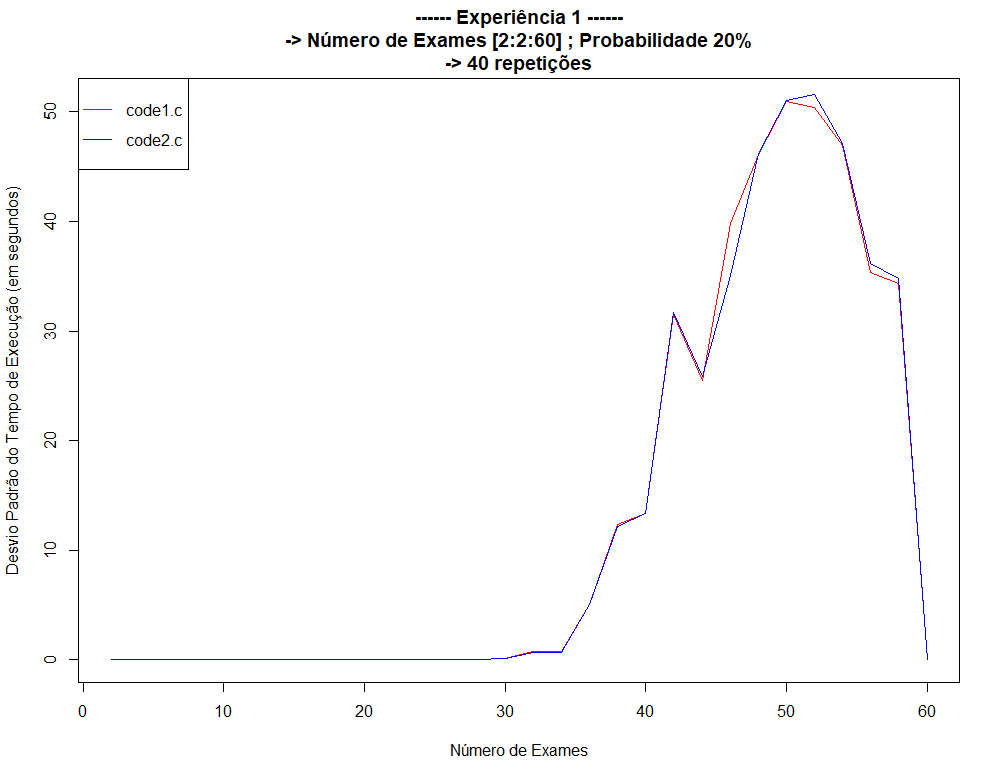
\includegraphics[width=7.3cm]{1_desvio.png} }}%
    \caption{Experiência 1}%
    \label{fig:example}%
\end{figure}

Após a análise de algumas experiências com base no aumento do Número de Exames, mantendo o valor da Probabilidade (p) fixa, avançámos para as experiências opostas, isto é, onde variamos a Probabilidade (p) mantendo o valor do Número de Exames fixo. Os resultados desta experiência encontram-se representados na \textbf{Figura 3}. Neste caso é possível observar uma subida dos valores do tempo de execução muito mais brusca, isto é, com declive superior, quando comparado ao que acontece quando se varia o Número de Exames. O comportamento do valor do desvio padrão é semelhante ao observado nas experiências anteriores, possívelmente pelos mesmos motivos.


\begin{figure} [!htbp]
    \centering
    \subfloat[\centering Evolução do tempo de execução]{{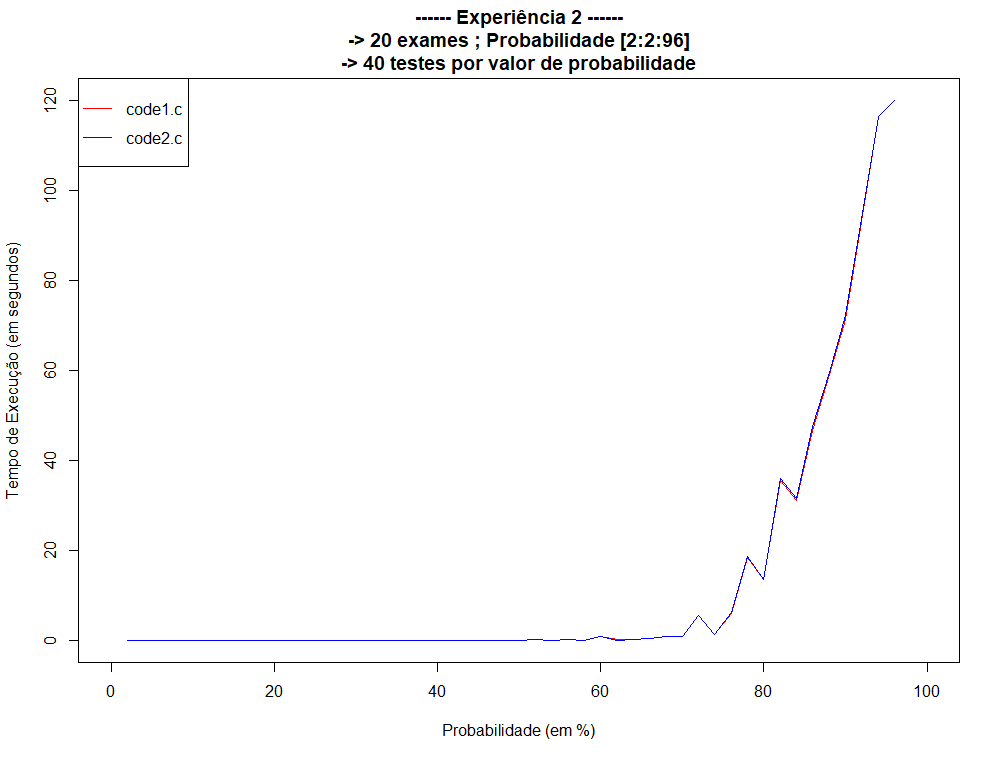
\includegraphics[width=7.3cm]{2_media.png} }}%
    \qquad
    \subfloat[\centering Evolução do desvio padrão]{{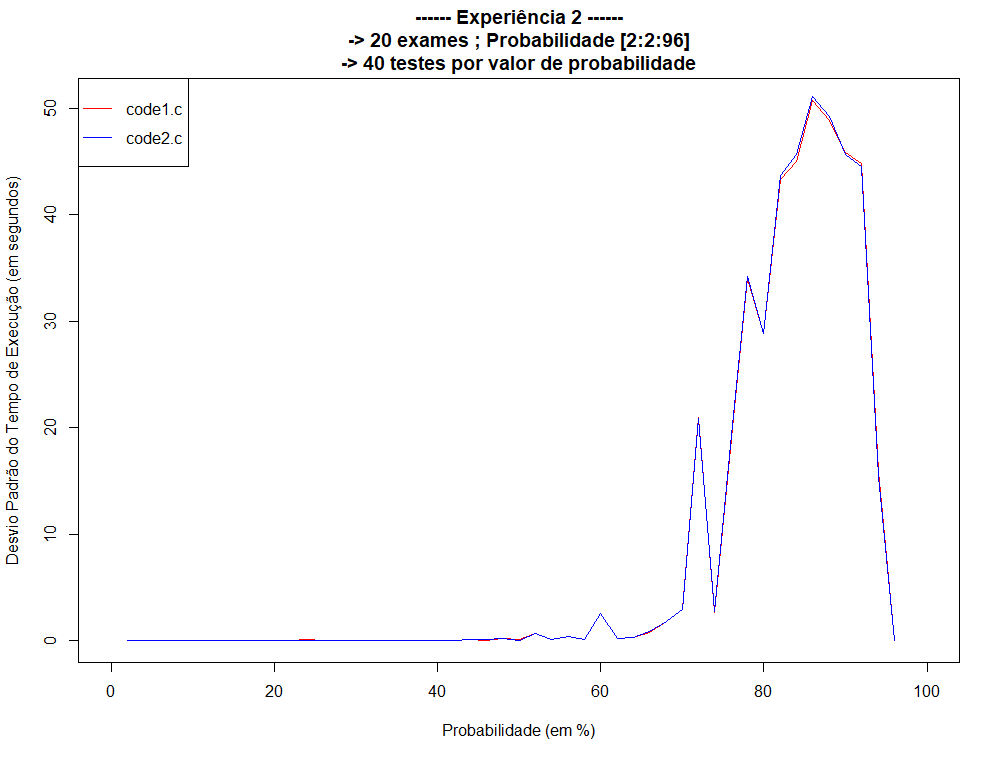
\includegraphics[width=7.3cm]{2_desvio.png} }}%
    \caption{Experiência 2}%
    \label{fig:example}%
\end{figure}

Como mencionado anteriormente, a experiência 3 foi realizada com o objetivo de observarmos com mais detalhe a curva ascendente que encontramos no gráfico \textbf{(a)} da \textbf{Figura 2}. Como seria de esperar, no gráfico \textbf{(a)} da \textbf{Figura 4}, observamos claramente o crescimento dos dados como se tivessemos feito \textit{zoom} no gráfico da primeira experiência. O desvio padrão continua bastante elevado mas, ao haver uma aproximação ao valor máximo de tempo de execução, os resultados irão tender a estabilizar, e, consequentemente, também o desvio padrão irá diminuir, como seria de esperar havendo este limite estipulado.\par

Da mesma forma que procedemos para a primeira experiência, de modo a observar melhor uma secção específica dos valores, voltámos a realizar com mais detalhe a experiência onde variamos apenas o valor da Probabilidade (p), desta vez entre 65\% e 95\% com incremento unitário, e obtivemos os resultados representados no gráfico \textbf{(b)} da \textbf{Figura 4}. Novamente verificamos que o valor do tempo de execução cresce muito rápidamente à medida que o valor da Probabilidade (p) também aumenta. A diferença para o gráfico \textbf{(a)} da \textbf{Figura 3} é que apenas testámos os valores de probabilidade a partir de 65\% o que nos permite visualizar com mais detalhe essa área em específico mas não oferece qualquer informação adicional para além do que obtivémos na experiência 2. Importante mencionar que na experiência 4 em específico decidimos experimentar aumentar o valor do tempo máximo de execução para 180 segundos e observar se tinha efeito nos gráficos mas é possível verificar que não existe diferença para além do facto do valor da variável dependente atingir valores superiores. A partir desta pequena alteração também podemos constatar que ao aumentar o limite máximo, os valores para o tempo de execução continuam a subir, seguindo o mesmo comportamento observado para valores inferiores.

\begin{figure} [!htbp]
    \centering
    \subfloat[\centering Experiência 3]{{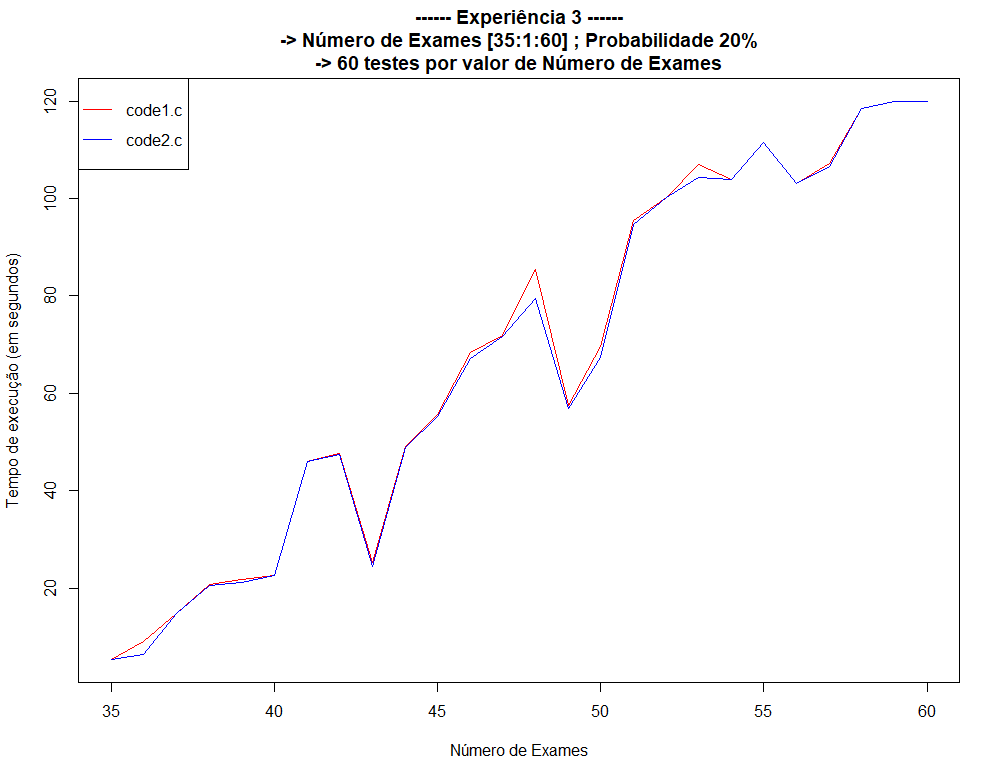
\includegraphics[width=7.3cm]{3_media.png} }}%
    \qquad
    \subfloat[\centering Experiência 4]{{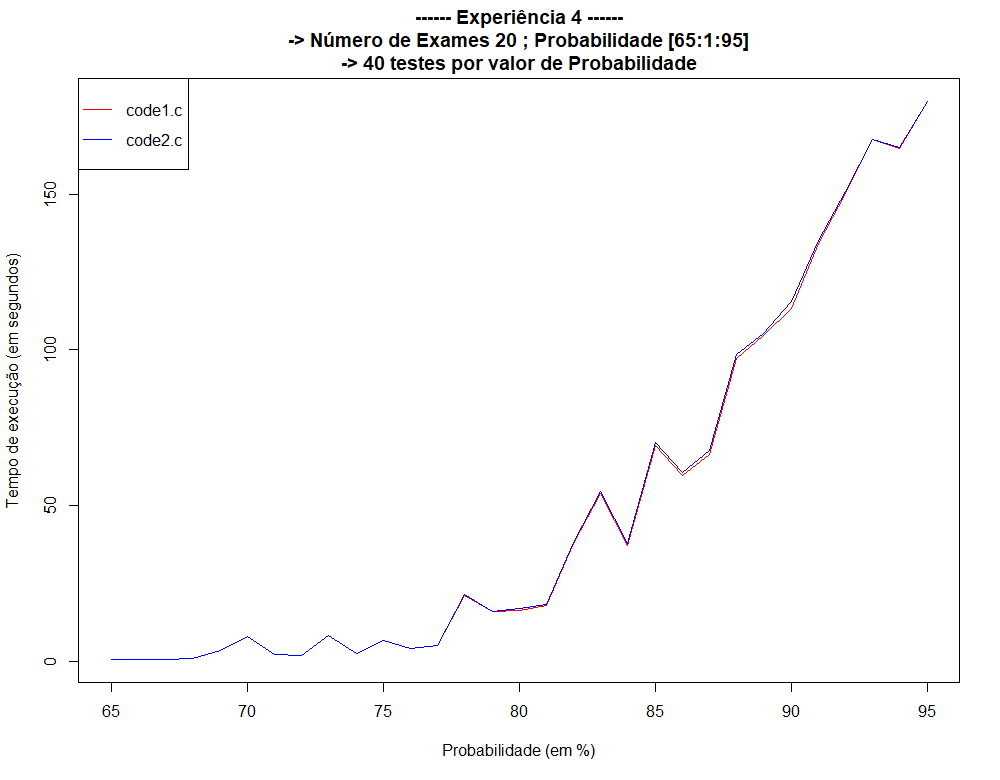
\includegraphics[width=7.3cm]{4_media.png} }}%
    \caption{Experiências 3 e 4}%
    \label{fig:example}%
\end{figure}

As experiências 1 a 4 foram todas realizadas mantendo o valor de uma das variáveis independentes fixo enquanto iamos aumentando o valor da outra variável independente, por outro lado, nas experiências 5 e 6 foram sendo incrementadas ambas as variáveis de forma a observar o comportamento resultante. Na experiência 5, o valor do Número de Exames foi variado entre 10 e 60 (2 em 2) e o valor da Probabilidade (p) variado pelos valores do vetor [2, 5, 15, 25, 50]\%. Ao visualizarmos os resultados desta experiência, conseguimos observar que a curva era agora mais suave do que no gráficos gráficos apresentados anteriormente. Como também existe uma variação do valor da Probabilidade (p) nesta experiência, poderiamos representar graficamente a sua influência na variável dependente, no entanto, como apenas iteramos sobre cinco valores distintos para esta variável independente, o gráfico que iriamos obter teria muito pouca resolução no sentido de que apenas teriamos cinco pontos representados.\par

A experiência final (Experiência 6) foi realizada com valores muito reduzidos de Probabilidade (p) de forma a observar o comportamento do gráfico para os valores iniciais da mesma, de 1\% a 16\%. O gráfico proveniente dos resultados desta experiência mostrou-se ser muito parecido aos gráficos cujos valores de Probabilidade (p) eram mais elevados. Decidimos não incluir a sua representação gráfica neste relatório pelo facto de não acrescentar nenhuma novidade às análises feitas anteriormente através das outras experiências.\par

Como fomos observando ao longo das seis experiências realizadas, todos os gráficos parecem apresentar um desenho que se assemelha a uma curva exponencial. Deste modo partimos para uma análise mais detalhada dos mesmos, experimentando calcular a reta de regressão linear para cada uma das experiências utilizando o método da transformação do eixo da variável dependente. Assim, é possível avaliar, através do cálculo de valores como o \(r^2\), a qualidade do ajuste das retas aos resultados obtidos e, caso estas se ajustem bem aos dados, poderemos afirmar que os resultados seguem uma distribuição exponencial. Ao aplicar a função logaritmo aos valores da variável dependente (tempo de execução do programa) de cada experiência, foi possível calcular os valores de \textbf{\textit{a}} e \textbf{\textit{b}} da expressão \(y = a+bx\) da reta de regressão linear. Este cálculo foi feito com recurso às funções \textit{lm()} e \textit{summary()} do \textit{R}, devolvendo os valores de \textbf{\textit{a}} e de \textbf{\textit{b}}, permitindo, assim, desenhar as retas visíveis na \textbf{Figura 5}. A segunda função mencionada devolve também o valor de \(r^2\) que se encontra representado em cada gráfico.\par
Os gráficos da \textbf{Figura 5}, como mencionado acima, mostram as retas de regressão linear que se ajustam a cada conjunto de dados. É possível verificar nos gráficos \textbf{(a)} e \textbf{(c)} que as retas se ajustam bastante bem aos dados, apresentando valores para \(r^2\) muito perto de 1. No caso do gráfico \textbf{(a)}, referente à experiência 1, obtiveram-se valores para o \(r^2\) superiores a 0.96 o que consideramos ser um ajuste bastante bom o que nos indica que o conjunto de dados segue, muito provavelmente, uma distribuição exponencial. O mesmo acontece para o gráfico \textbf{(b)} correspondente à experiência 2, onde se obtiveram valores para o \(r^2\) superiores a 0.95. Isto indica que tanto o crescimento do Número de Exames como o crescimento do valor da Probabilidade (p) provocam um crescimento exponencial da variável dependente, o tempo de execução do problema. Os gráficos \textbf{(b)} e \textbf{(d)} dizem respeito às experiências 3 e 4, respetivamente, que foram realizadas com o intuíto de analisar mais detalhadamente uma determinada secção dos gráficos obtidos inicialmente para as experiências 1 e 2. Os valores de \(r^2\) obtidos nestas regressões são inferiores aos obtidos nas regressões já analisadas pelo facto do conjunto de dados se focar apenas num conjunto pequeno para valores da variável independente em estudo e, deste modo, não existir tanta informação sobre o comportamento dos resultados para valores iniciais destas variáveis o que causa esta maior diferença aquando da analise da regressão linear.

\begin{figure} [!htbp]
    \centering
    \subfloat[]{{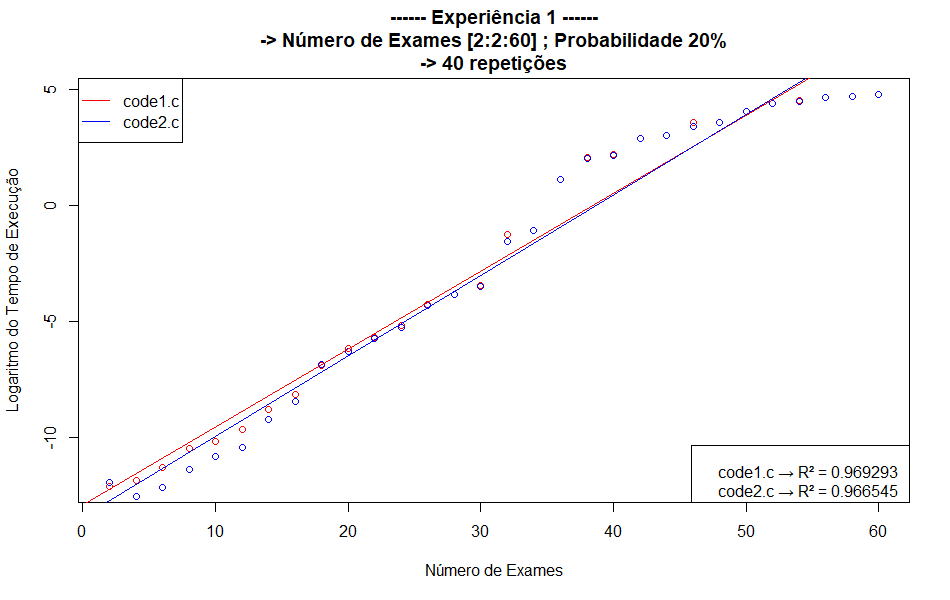
\includegraphics[width=7.5cm]{1_regressao.png} }}%
    \subfloat[]{{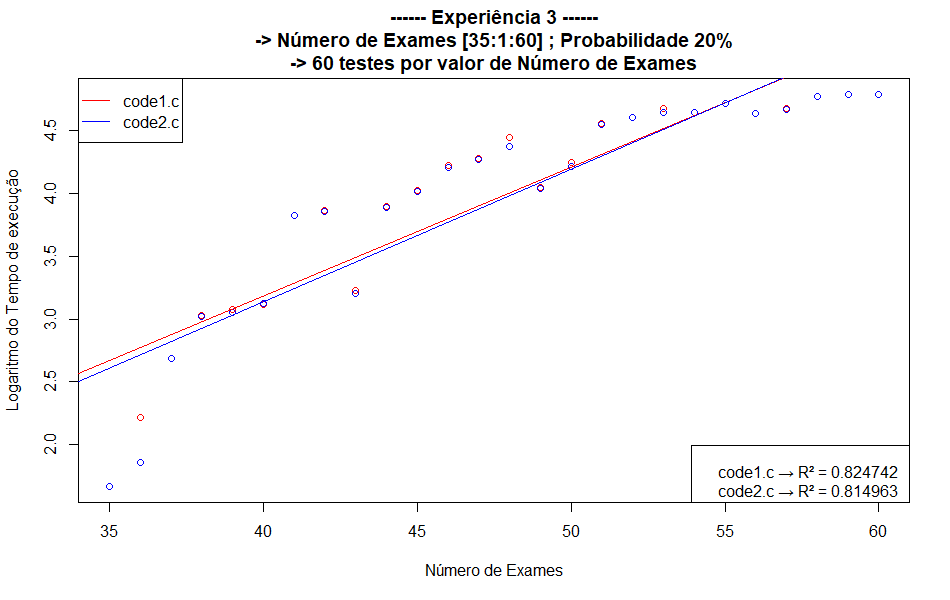
\includegraphics[width=7.5cm]{3_regressao.png} }}%
    \qquad
    \subfloat[]{{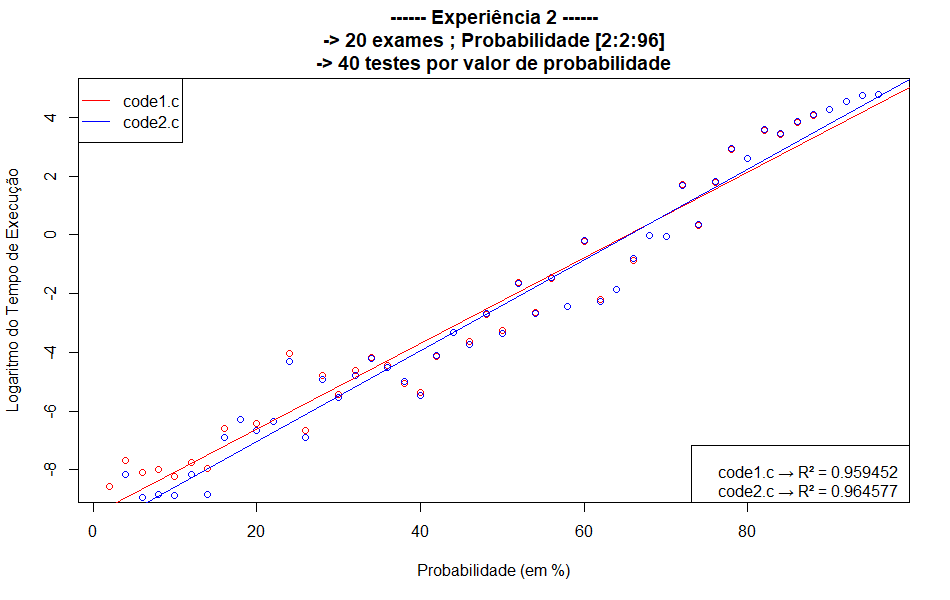
\includegraphics[width=7.5cm]{2_regressao.png} }}%
    \subfloat[]{{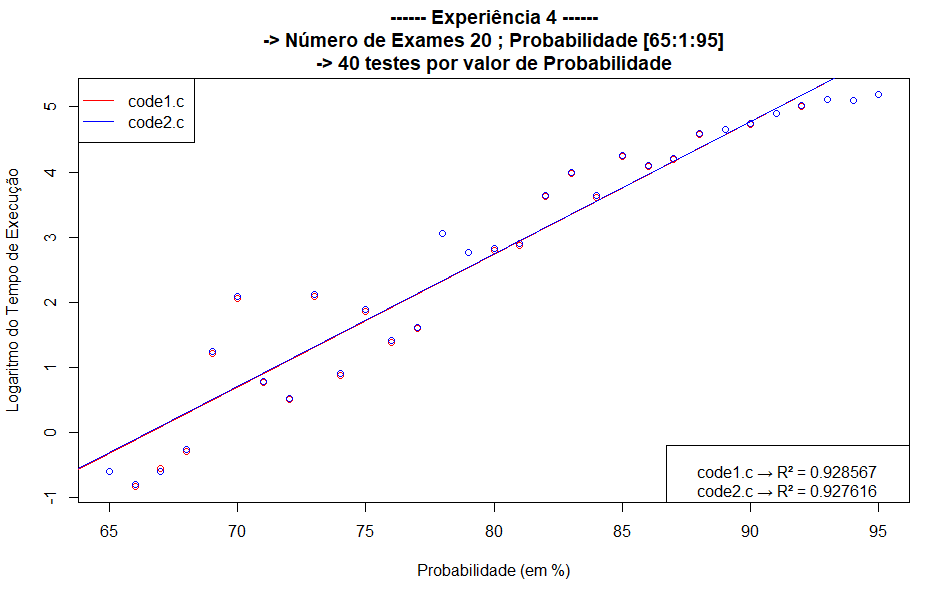
\includegraphics[width=7.5cm]{4_regressao.png} }}%
    \caption{Regressões lineares - Experiências 1 a 4}%
    \label{fig:example}%
\end{figure}

\par
Para terminar esta secção de análise dos resultados obtidos, não poderiamos deixar de mencionar que em todos os gráficos apresentados são representados, através de cores distintas, os resultados de ambos os programas fornecidos (\textit{code1.c} e \textit{code2.c}). Não observámos nenhuma vantagem singificativa na utilização de cada programa, no entanto, podemos verificar nos gráficos das \textbf{Figuras 2} a \textbf{4} que, por vezes, a linha de cor azul (correspondente ao \textit{code2.c}) encontra-se abaixo da linha de cor encarnada e, portanto, isso significa que obteve resultados muito ligeiramente inferiores. No entanto acreditamos que esta ligeira diferença seja insignificante pelo facto de ser tão pequena e de não revelar ser de grande importância em nenhum caso testado.

\section{Conclusões}
\paragraph{}
No final da observação e análise mais detalhada de cada experiência realizada conseguimos retirar algumas conclusões acerca do comportamento destes programas. Nomeadamente conseguimos observar o efeito que o  \textbf{Número de Exames} e o valor da  \textbf{Probabilidade  (p)} têm no \textbf{Tempo de Execução} dos programas, que era o nosso objetivo inicial. Através da análise da representação gráfica dos resultados obtidos e a aplicação de regressões lineares, observámos que esta relação entre as variáveis independentes e a variável dependente segue uma distribuição exponencial.\par
Outro ponto a frisar é que, o facto de não termos encontrado uma diferença significativa entre os programas fornecidos nas nossas experiências, não nos permite concluir que esta não exista pois poderiam surgir resultados diferentes com a realização de mais testes com outros valores para as variáveis independentes que não explorámos.\par
Por fim, consideramos que o trabalho realizado foi de encontro ao proposto pelo enunciado desta meta do trabalho prático e que conseguiu, nesta fase inicial, dar-nos uma visão melhor do problema em causa e de como as variáveis estudadas podem afetar os resultados destes programas.

\section{Trabalho Futuro}
\paragraph{}
Com a realização deste relatório e de todas as experiências nele contigo, ficamos agora com uma ideia melhor deste problema que nos permite começar desde já a pensar como iremos proceder nas restantes metas e que comportamento podemos esperar destes programas. Apesar de termos realizado seis experiências, achamos que poderiamos benificiar de mais, caso existisse tempo para tal, de forma a melhorar ainda mais os dados obtidos.

\end{document}